\chapter{Data Analysis}

\section{Efficiencies}
\paragraph{}The High resolution spectrometers are capable of detecting a myriad of particles that track through the detectors. The designed of an experimental trigger uses the properties of the individual detectors to capture data of the meaningful events. Many accidentals, back ground, and unwanted events trigger the data acquisition system. The removal of these unwanted events take place during analysis via software cuts. Restricting the applicable signal from certain detectors through different cuts allows for the rejection of back ground particles and prevents contamination in the yield extraction. 

\subsection{Particle Identification Efficiency}
\paragraph{} One of the largest sources of contamination for the MARATHON experiment is negatively charge pions. These pions are removed through software cuts made in the total signal from the ten cherenkov PMTs(photomultiplier tubes) and the energy deposited into the blocks of both layers of the calorimeter. Electrons can be identified by their behavior in the spectrometer. High quality electrons will track through the entire detector stack to deposit most of their energy into the total calorimeter system and creating a large amount of light in the cherenkov. Though this knowledge tight cuts can be used to study the efficiency of the particle identification system. Plotting the signal in the cherenkov versus the energy deposited into both layers of the calorimeter allow for visual representation of the sampling cuts made in the efficiency studies, which can be seen in figure \ref{elesample}. 

\begin{figure}[h]
	\centering

	\textbf{Cherenkov sum versus Total Energy deposited }\par\medskip
	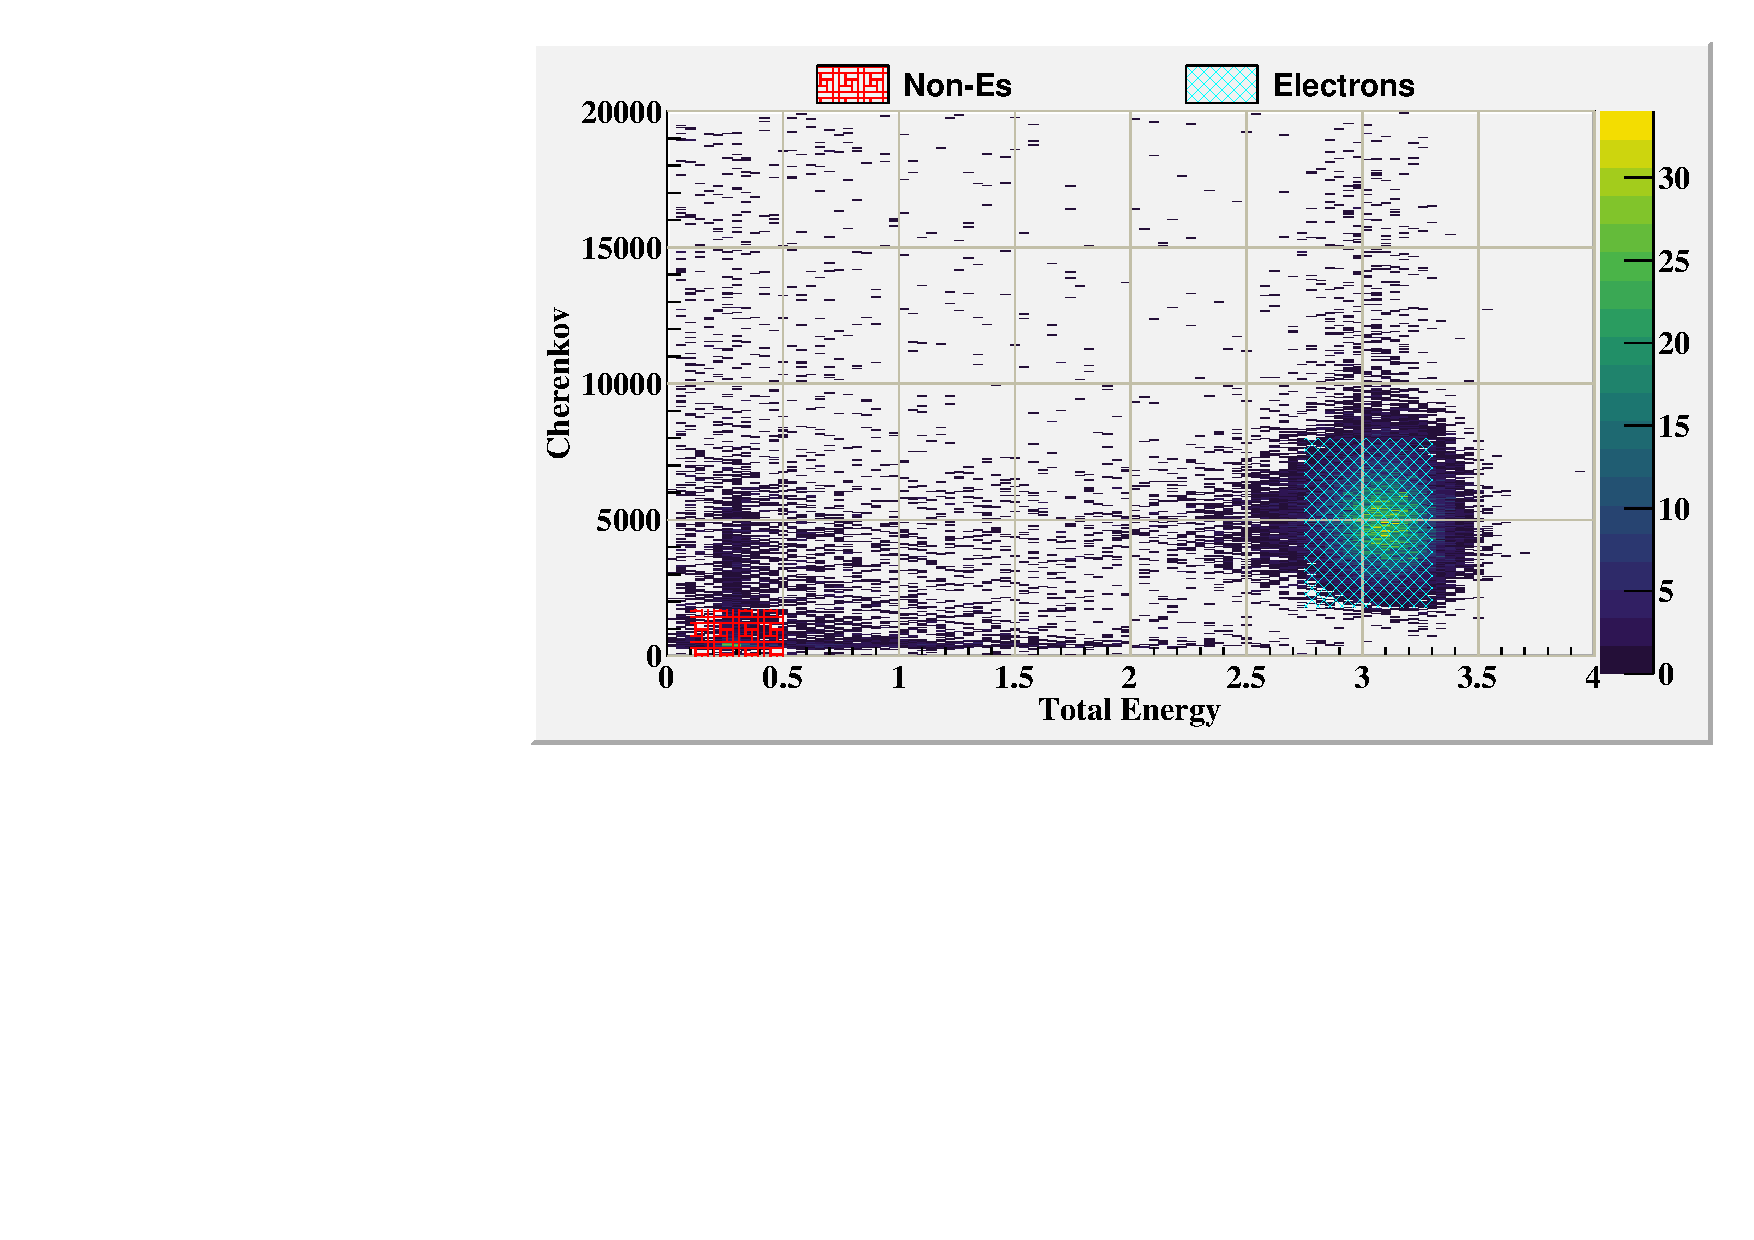
\includegraphics[width=13cm]{PID_2d}
	\caption{Two dimensional plot of the cherenkov sum versus Total Energy deposited, including electron sampling in teal and non-electron sampling in red. }
	\label{elesample}
\end{figure}

\begin{equation}\label{effequ}
\begin{split}
		GE_{sample} & = \textrm{Known electron sample from tight cut}  \\
	      GE_{pass} & = \textrm{$GE_{sample}$ and pass indentification cut} \\
	Electron_{eff}  & = \frac{ GE_{pass} } { GE_{sample} } 
\end{split}
\end{equation}
\paragraph{}The efficiency of the spectrometer's particle identification(PID) detectors was determined by using the first calorimeter layer, the second calorimeter layer, and the cherenkov to provide a samples of good electrons and other particles. The PID efficiency of the individual detectors were determined using equation \ref{effequ}. The good electron sample for calculating the efficiency of the single detector was defined by sampling through the other two detectors. Sampling through the two layers of the calorimeter is shown in figure \ref{Prl1Prl2}. The cherenkov good electron sample shown in figure \ref{cersam}. The electron sample from the cherenkov is contaminated by delta particles that are created by secondary scattering events from pions and a combination of unknown particles titled $X1$. The $X1$ events do not deposit enough energy into the calorimeter system to be consider as good electrons that scatter from our target. Using sampling in one layer of the calorimeter and the cherenkov, these unwanted low energy particles are rejected from sampling for efficiency calculations. 


\begin{figure}[]
{\centering
\textbf{Particle ID and efficiency sampling for the two layers of the calorimeter }\par\medskip}
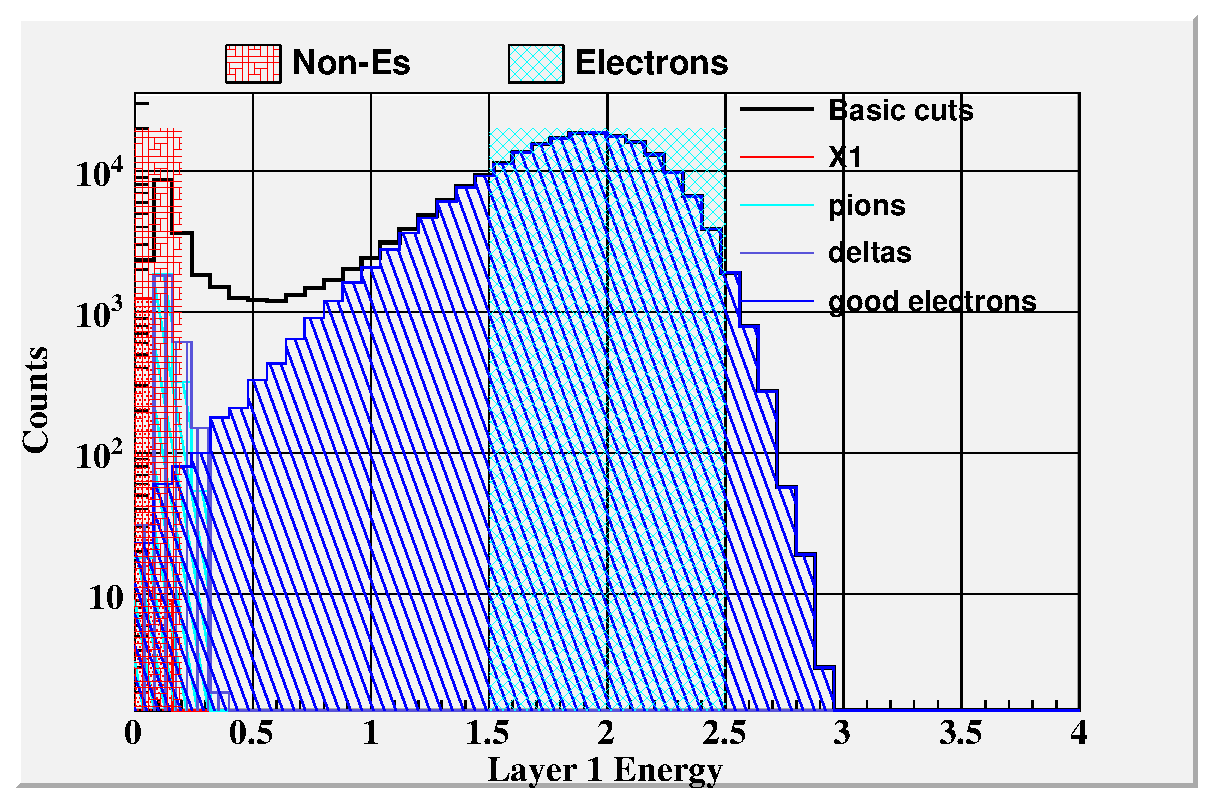
\includegraphics[width=8.5cm]{Lplr1}
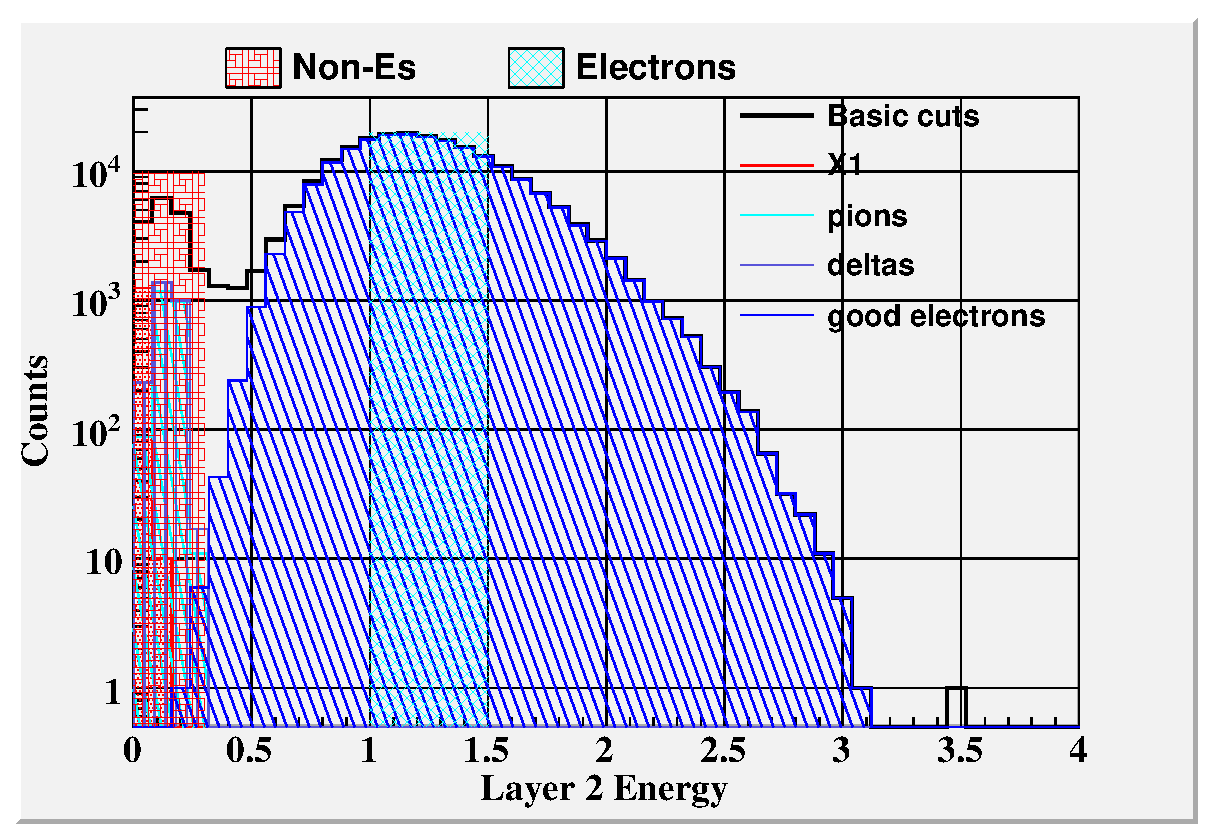
\includegraphics[width=8.5cm]{Lprl2}
\caption{Electrons and other back ground particles identified via cuts in the total calorimeter and the gas cherenkov shown in the individual layers of the calorimeters. Sampling cuts for Electrons in teal and Non-Electrons in red.}
\label{Prl1Prl2}
\end{figure}

\begin{figure}[]
{\centering
\textbf{Particle ID and efficiency sampling for Cherenkov }\par\medskip}
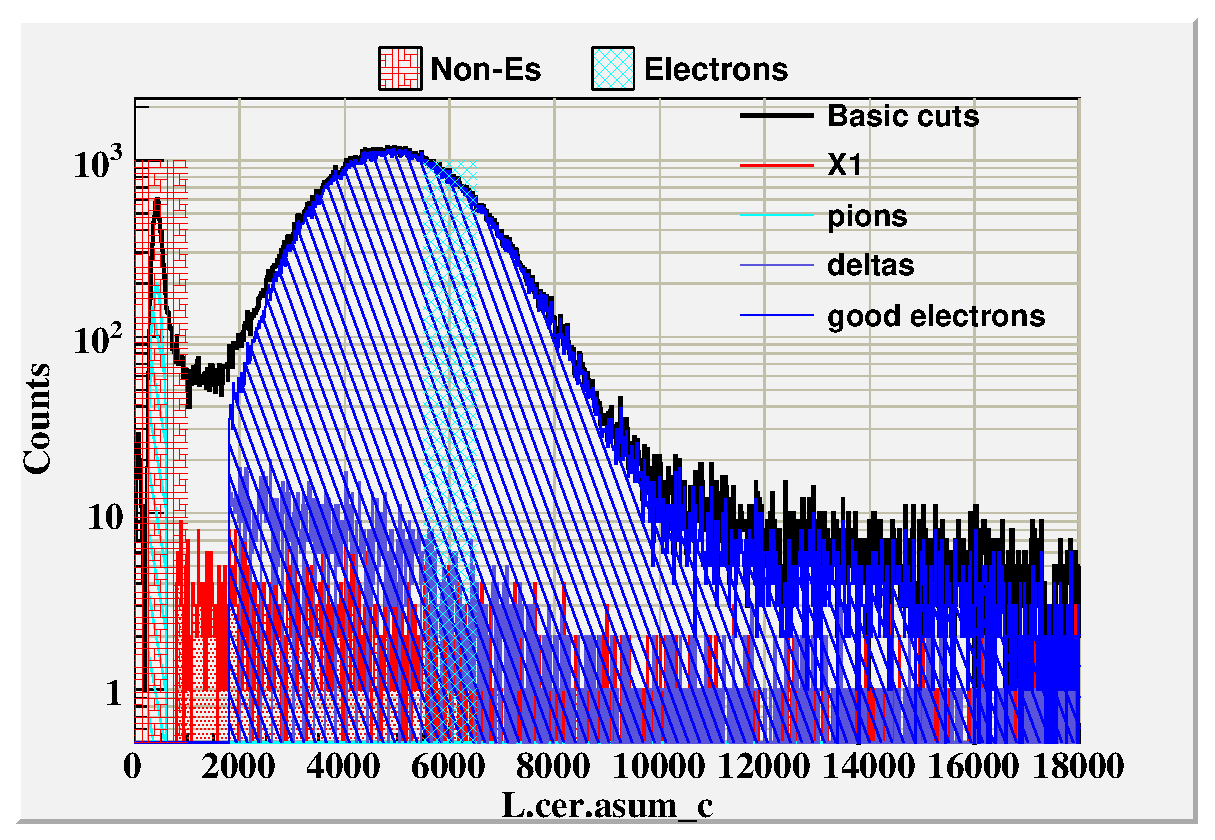
\includegraphics[ width=17cm]{Lcerasum}
\caption{Electrons and other back ground particles identified via cuts in the total calorimeter and the gas cherenkov shown in the sum of the gas cherenkov.Sampling cuts for Electrons in teal and Non-Electrons in red.}
\label{cersam}
\end{figure}
